\scanpage{59}
% archive sheet number: 58

% L1–6, overlap of neighbourhoods
$x\in U\cap U'\cap Y_1$ \deleted{donc} dans un voisinage $W_1$ de $U\cap U'\cap Y_1$, et $\unsure{\varphi|\phi}_{2\deleted{\unsure{1}}x}=\varphi'_{2x}\,(=f_{2x})$ \deleted{pour $x$ dans i.e. $\varphi_{1x}=\varphi$} pour $x\in U\cap U'\cap Y_2$, donc $\varphi_{1x}=\varphi'_{1x}+1$ pour $x\in U\cap U'\cap Y_2$, donc pour $x$ dans un voisinage $W_2$ de $U\cap U'\cap Y_{2}$. Donc si $x\in W_1\cap W_2$, on aura \deleted{\unsure{al.}} à la fois

% L7, two equalities
\[
\varphi_{1x}=\varphi'_{2x}\qquad\text{et}\qquad\varphi_{1x}=\varphi'_{1x}+1
\]

% L8–9, contradiction
i.e. $0=1$, absurde [compte tenu que $W_1\cap W_2\ne\varnothing$, $X$ étant irréductible].

% L10–11, below rule
Utilisant cet exemple, on trouve un exemple avec $Y$ \uline{irréd} (de \uline{dim 2} \inserted{ds $X$ de dim 3}],

% L12–16, new construction
Pour ceci, dans $X$ on \unsure{considère|considèrera|considérant} un $X_1$ \inserted{fermé (dim 2)} qui recoupe $Y$ suivant la figure $Y_1=X_1\cap Y$ précédente

% L13–15, left plane
\figure{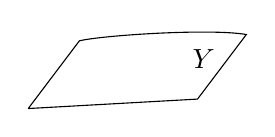
\begin{tikzpicture}[x=1cm,y=1cm]\draw (0,0)--(2.15,.12)--(2.77,.94) .. controls (2.31,1.02) and (.94,.93) .. (.65,.86)--(0,0);\node at (2.23,.63) {$Y$};\end{tikzpicture}}

% L16, inline pair of curves
\figure{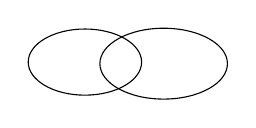
\begin{tikzpicture}[x=1cm,y=1cm]\draw (0,0) ellipse (.72 and .42);\draw (1.00,-.02) ellipse (.81 and .45);\end{tikzpicture}}

% L16–18, foot
. On prend alors le faisceau $F$ sur $X$ extension \unsure{can|can.} du faisceau des applications de $X_1$ dans $\mathbb{Q}$.
